\begin{figure}
\begin{center}
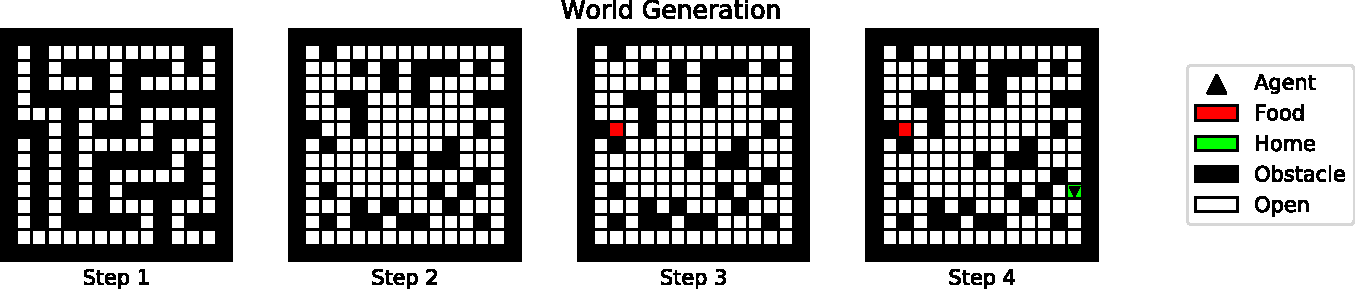
\includegraphics[width=\textwidth]{img/world_explanatory}
\caption{
Environment generation procedure, Left to Right: First, an $n \times m$ matrix is filled with walls. The walls are removed systematically to form a maze structure. Next, a percentage of the maze's walls are removed creating open space. Finally, a food marker and home marker are placed within the environment. The agent is placed on the home marker, facing a random direction.
}
\label{fig:world_explanatory}
\end{center}
\end{figure}
